\subsection{Contrôle d'essaim}

\begin{frame}[c]{Approches de contrôle}
    \vfill
    \begin{columns}[c,totalwidth=\textwidth]
        \column{0.5\textwidth}
        \textbf{Contrôle centralisé}
        \begin{itemize}
            \item[\textcolor{green}{+}] Précision élevée
            \item[\textcolor{green}{+}] Calcul global simplifié
            \item[\textcolor{red}{-}] Dépendance aux communications
        \end{itemize}
        
        \column{0.5\textwidth}
        \textbf{Contrôle décentralisé}
        \begin{itemize}
            \item[\textcolor{green}{+}] Robustesse
            \item[\textcolor{red}{-}] Coordination complexe
        \end{itemize}
    \end{columns}
    
    \vspace{0.5cm}
    \textbf{Stratégie eSWARM :}
    \begin{enumerate}
        \item Implémentation centralisée (simplicité)
        \item Évolution vers une approche décentralisée
    \end{enumerate}
    \vfill
    
    \vspace{0.3cm}
    \footnotesize{\cite{jamshidpey_centralization_2024}}
\end{frame}

\begin{frame}[c]{Méthodes de contrôle d'essaim}
    \vfill
    \begin{columns}[c,totalwidth=\textwidth]
        \column{0.6\textwidth}
        \textbf{Algorithmes principaux :}
        \vspace{0.3cm}
        \begin{itemize}
            \item \textbf{Loi de consensus} \cite{ali_practical_2018, koung_consensus-based_2020} :
            \begin{itemize}
                \item $u_i(t) = \sum_{j=1}^{n} a_{ij}(t) [x_j(t) - x_i(t)]$
            \end{itemize}
            \vspace{0.3cm}
            \item \textbf{Leader-follower} \cite{loria_leaderfollower_2016, yang_adaptive_2021} :
            \begin{itemize}
                \item Hiérarchie avec robots leaders et followers
            \end{itemize}
            \vspace{0.3cm}
            \item \textbf{Changement de modèle} \cite{inglett_object_2017} :
            \begin{itemize}
                \item Détermination d'une nouvelle dynamique
            \end{itemize}
        \end{itemize}
        
        \column{0.4\textwidth}
        \begin{figure}
            \centering
            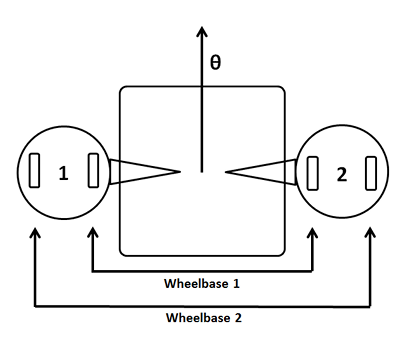
\includegraphics[width=\linewidth]{3-etat-de-lart/pic/changement modele.png}
            \caption{Changement de modèle}
        \end{figure}
    \end{columns}
    \vfill
    
\end{frame}



%%\textbf{Classification \cite{oh_survey_2015} :}
%%    \begin{itemize}
 %       \item \textbf{Contrôle par position} : coordonnées globales, ajustement actif
 %       \item \textbf{Contrôle basé sur le déplacement} : positions relatives sans position absolue
 %       \item \textbf{Contrôle basé sur la distance} : référentiels locaux uniquement
 %   \end{itemize}